% !TEX root = ../lust-1.tex
%
\chapter{Selbstmanagement}
\label{sec:selbstmanagement}

\paragraph{Teil 2 der Hausarbeit}
Suchen Sie sich 5 für Sie relevante Ziele aus und setzen Sie Prioritäten mit Hilfe der im Modul vorgestellten Kriterien. Begründen Sie Ihre Entscheidung. \\[4em]

Wie im Kurs erläutert ist es wichtig die Verhaltensweisen, welche erreicht werden wollen, zunächst konkret zu formulieren. Für die Aufgabe werden die folgenden persönlichen Ziele näher betrachtet: Das Fertigstellen der in der vorherigen Aufgabe beschriebenen Webseite, die persönliche Bestzeit beim Maisel´s FunRun Halbmarathon zu verbessern, das abschließen des Informatik-Studiums, die bereits begonnene Buchreihe “Der schwarze Turm” von Steven King zu ende zu lesen und das eigene Schlafzimmer zu renovieren.

Um die Ziele im Anschluss genauer zu analysieren und priorisieren zu können wird das Teile-und-Herrsche Prinzip (engl. “Divide-and-Conquer”) angewendet und in die folgenden 3 Fragen zerlegt \cite{WEB:VHB:LuSt1:Zielhierarchien}:

\begin{itemize}
    \item Was muss gemacht werden?
    \item Wann muss es gemacht werden?
    \item Was ist jetzt wichtig, was eher nicht?
\end{itemize}

\subsubsection{1. Ziel: Fachschafts-Webseite erstellen}
Wie in der vorherigen Aufgabe beschrieben, soll der Webauftritt unserer Fachschaftsvertretung erneuert werden. Konkretes Ziel ist hier eine neue Homepage, welche nach Möglichkeit mindestens denselben Funktionsumfang bzw. die selben Informationen beinhaltet.
Die Hierarchie könnte beispielsweise folgendermaßen dargestellt werden:

\begin{figure}[htb]
	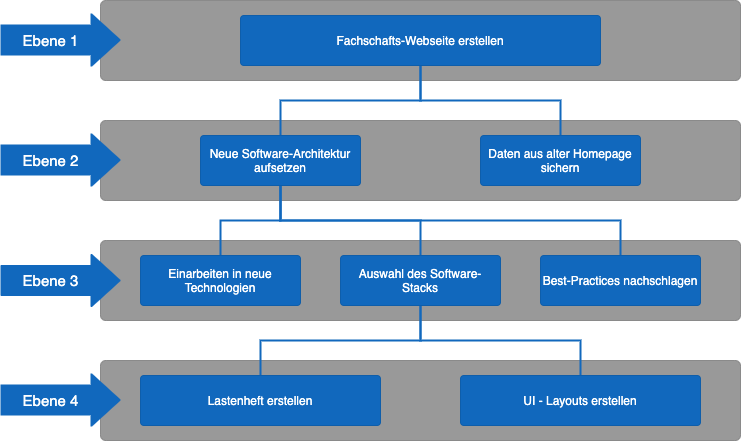
\includegraphics[width=\textwidth]{gfx/homepage}
	\caption{Zielhierarchie: \textit{Fachschafts-Webseite erstellen}}
\end{figure}

Da es sich hierbei um ein eher komplexes Thema handelt und evtl. die Zuarbeit von Kommilitonen benötigt ist der Zeitaufwand relativ hoch. Außerdem gibt es keinen festen Zeitpunkt zu dem das Projekt abgeschlossen sein muss, daher ist die Priorität eher niedrig.

\subsubsection{2. Ziel: Halbmarathon-Zeit verbessern}
Ein persönliches Ziel ist, die letztjährige Zeit beim “Maisel´s FunRun” Halbmarathon zu verbessern. Um dieses Ziel zu erreichen könnte man folgende Einteilung vornehmen:

\begin{figure}[htb]
	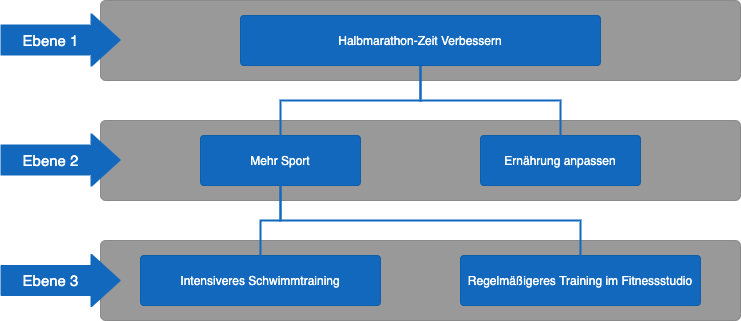
\includegraphics[width=\textwidth]{gfx/marathon}
	\caption{Zielhierarchie: \textit{Halbmarathon-Zeit verbessern}}
\end{figure}

Hier handelt es sich um einen langwierigen Prozess, für den gewisse Aufgaben regelmäßig wiederholt werden müssen. Diese können jedoch mit Hilfe von gutem Zeitmanagement in den Alltag integriert werden. Im Vergleich zum 1. Ziel existiert hier zwar ein fester Zeitpunkt, allerdings sind die Auswirkungen bei Erreichen eher gering. Aus diesem Grund ist die Priorität auch in diesem Fall eher niedrig.

\subsubsection{3. Ziel: Studium abschließen}
Dieses Ziel ist angelehnt an das Beispiel im Kurs, wurde allerdings deutlich konkretisiert. Um das Studium abzuschließen gilt es neben dem bestehen der beiden verbleibenden Module (Theoretische Informatik und diesem VHB Kurs) noch die Bachelorarbeit abzugeben. Da diese in Kooperation mit dem betreuenden Lehrstuhl und einem Unternehmen entsteht, existieren auch hier zusätzliche Abhängigkeiten:

\begin{figure}[htb]
	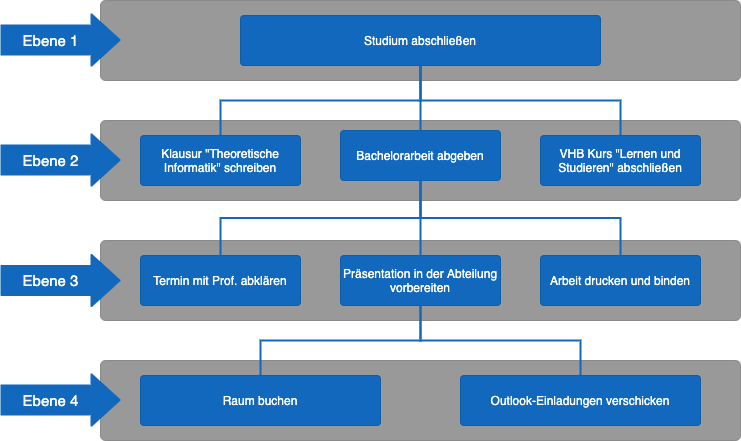
\includegraphics[width=\textwidth]{gfx/studium}
	\caption{Zielhierarchie: \textit{Studium abschließen}}
\end{figure}

Das Erreichen dieses Ziels hat sowohl deutliche Auswirkungen, als auch eine feste Deadline. In der hier aufgeführten Liste handelt es sich daher um das wichtigste und ist daher jenes Ziel mit der höchsten Priorität.

\subsubsection{4. Ziel: Buchreihe fertig lesen}
Zum herstellen einer vernünftigen Work-Life-Balance und um zu Vermeiden nur noch an Projekten für Arbeit und / oder Studium zu arbeiten wurde als persönliches Ziel festgehalten, die bereits begonnene Buchreihe “Der dunkle Turm” von Stephen King zu ende zu lesen.

\begin{figure}[htb]
	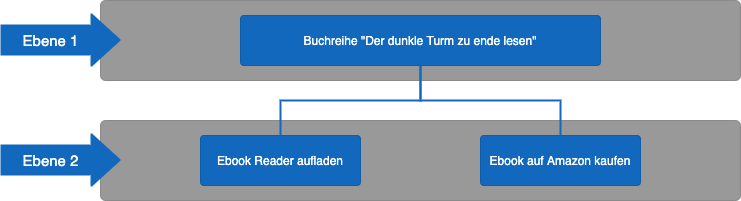
\includegraphics[width=\textwidth]{gfx/buchreihe}
	\caption{Zielhierarchie: \textit{Buchreihe fertig lesen}}
\end{figure}

Auch hier handelt es sich um ein Ziel mit keinem festen Zeitpunkt. Zudem ist hier sprichwörtlich eher “der Weg das Ziel”. Das heißt, die Auswirkungen beim tatsächlichen Erreichen sind sehr gering. Somit ist dieses Ziel, dasjenige welches die geringste Priorität in der Liste hat.

\subsubsection{5. Ziel: Schlafzimmer renovieren}
Um den eigenen Wohnkomfort zu erhöhen wurde das Ziel gefasst, im Schlafzimmer neuen Parkett-Boden zu verlegen und die Wände neu zu streichen.

\begin{figure}[htb]
	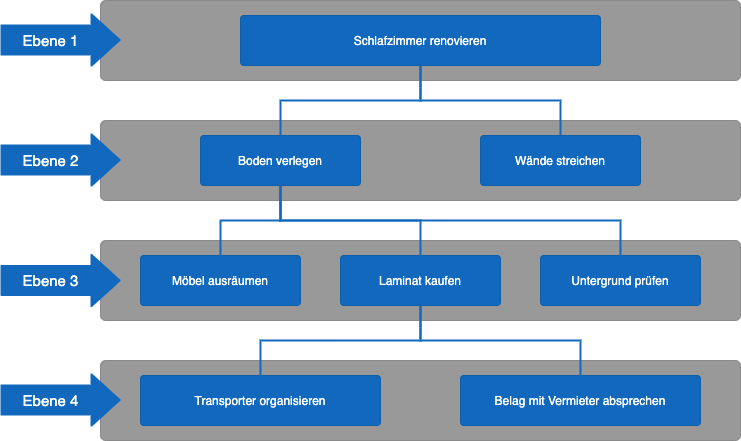
\includegraphics[width=\textwidth]{gfx/renovieren}
	\caption{Zielhierarchie: \textit{Schlafzimmer renovieren}}
\end{figure}

Dieses Ziel besitzt zwar ebenfalls keinen Zeitpunkt zu dem es zwangsläufig erreicht sein muss, jedoch hat es eine deutliche Auswirkung wenn die entsprechenden Aufgaben bzw. Arbeiten abgeschlossen wurden.Der Zeitaufwand hält sich außerdem verhältnismäßig in Grenzen, sodass dieses Ziel mit mittlerer Priorität bewertet wird.
